\documentclass[12pt]{article}
\usepackage[a4paper, margin=2.5cm]{geometry}
\usepackage{fontspec}
\usepackage{graphicx}
\usepackage{setspace}
\usepackage{titlesec}
\usepackage{tikz}
\usepackage{caption}
\usetikzlibrary{shapes.geometric, arrows.meta, positioning}

% === FONT ===
\setmainfont{Times New Roman}

% === STYLE ===
\setstretch{1.5}
\titleformat{\section}{\bfseries\large}{\thesection.}{0.5em}{}

% === TITLE INFO ===
\title{\textbf{Cognitive Psychology and Hierarchical Task Analysis
pada Game Monster Hunter World}}

\author{Muhamad Rizal - 11241049 \\
Mata Kuliah: IF2514502 - IMK}
\begin{document}

\maketitle

\section{Analisis Psikologi Kognitif}
\subsection{Persepsi}
\begin{figure}[h!]
    \centering
    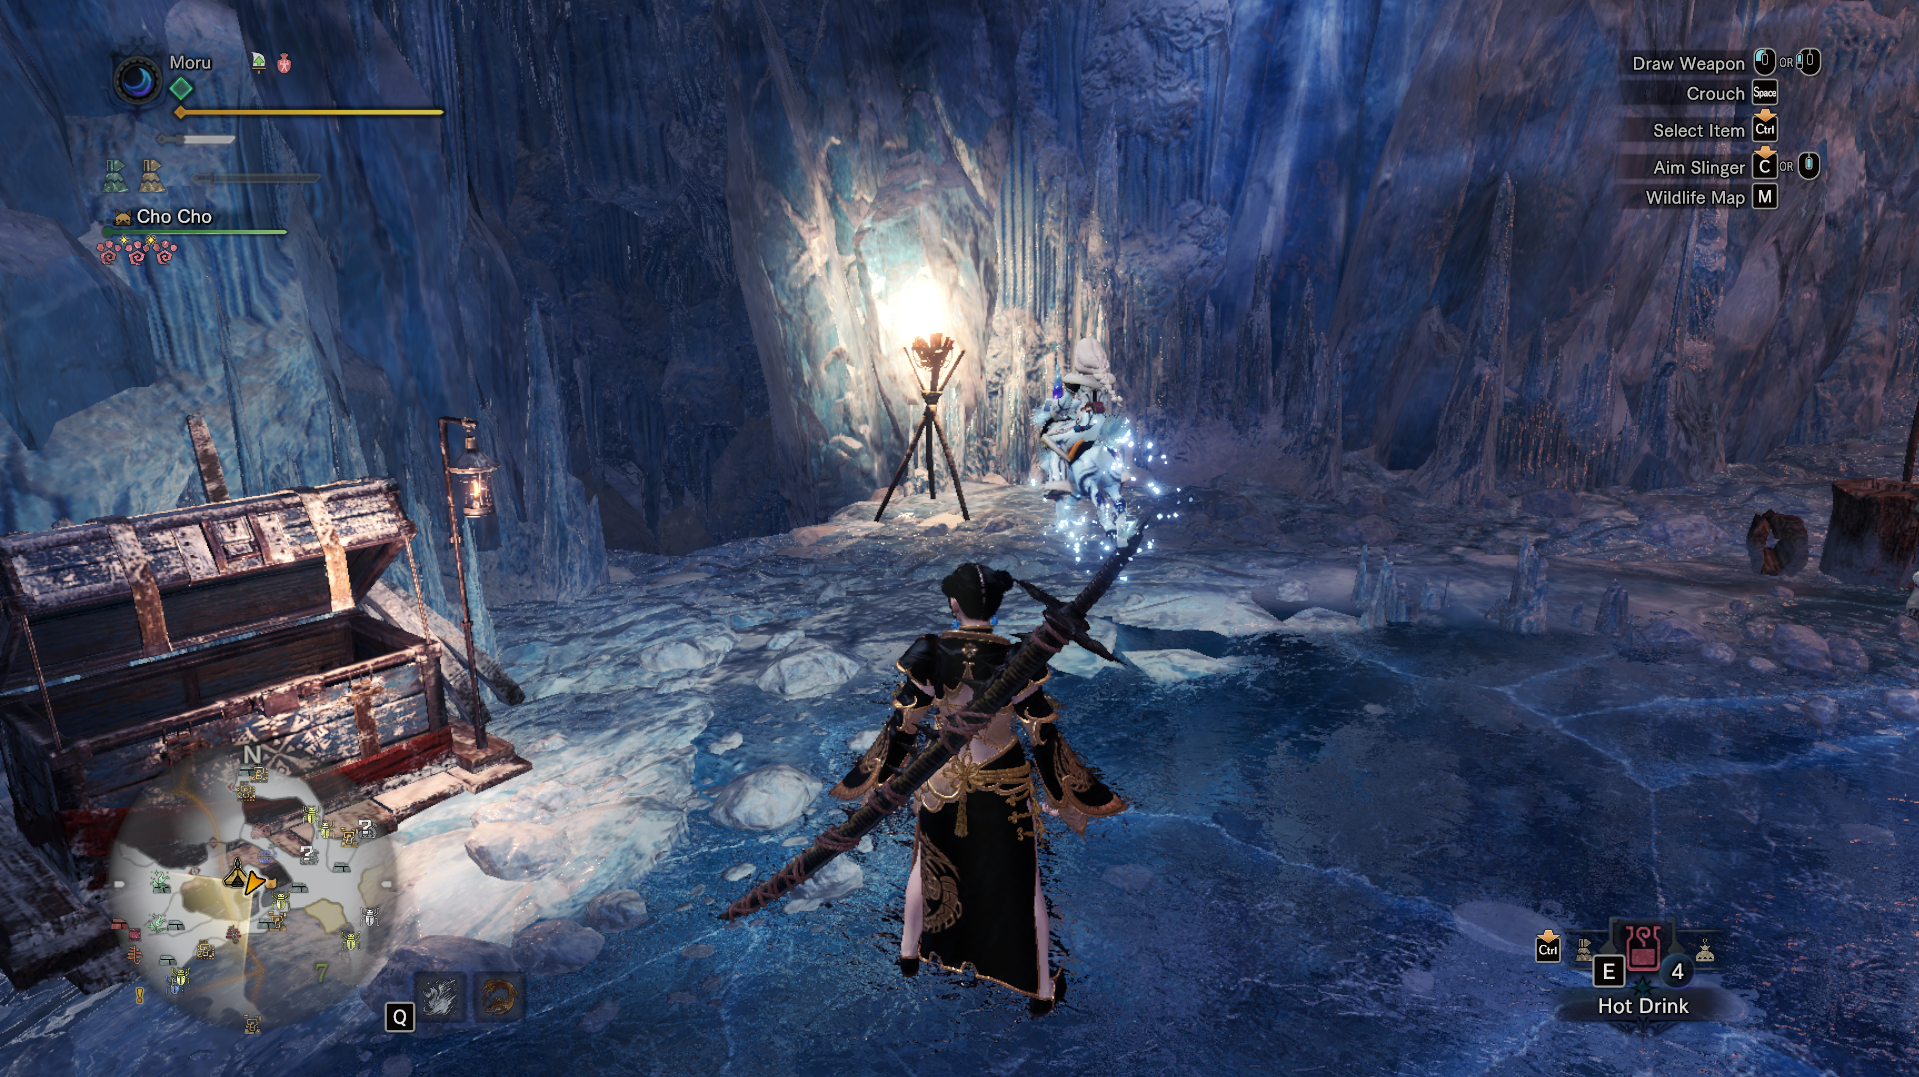
\includegraphics[width=0.8\textwidth]{Image/Main_Secreenshots.png}
    \caption{Tampilan HUD (Heads-Up Display) dalam Monster Hunter World}\label{fig:hud}
\end{figure}
Desain User Interface dalam game Monster Hunter: World menarik Persepsi pemain melalui penggunaan elemen visual dan warna yang Kuat seperti:
\begin{description}
    \item[Health Bar dan Stamina Bar] 
    Health Bar menunjukkan kondisi kesehatan karakter. Saat bar penuh, pemain merasa aman ketika berkurang dan berkedip merah, pemain langsung mempersepsikan kondisi bahaya. 
    Sedangkan Stamina Bar memberikan persepsi mengenai kemampuan untuk berlari, menyerang, atau menghindar.

    \begin{center}
    \begin{minipage}{0.45\textwidth}
        \centering
        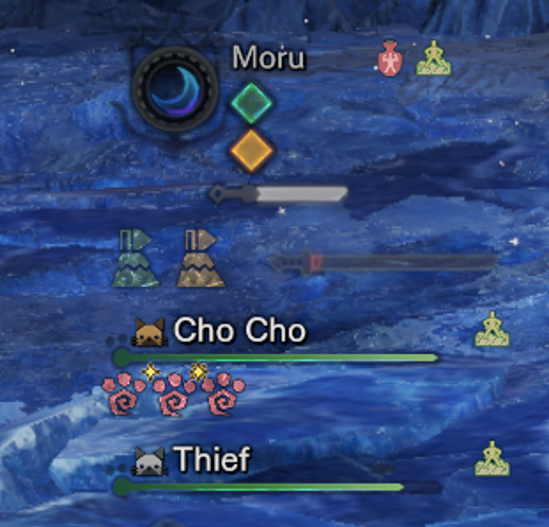
\includegraphics[width=\textwidth]{Image/HUD_Details/HP_Minimized.png}
        \captionof{figure}{Health Bar dan Stamina Bar dalam Compact Mode}
    \end{minipage}
    \hfill
    \begin{minipage}{0.45\textwidth}
        \centering
        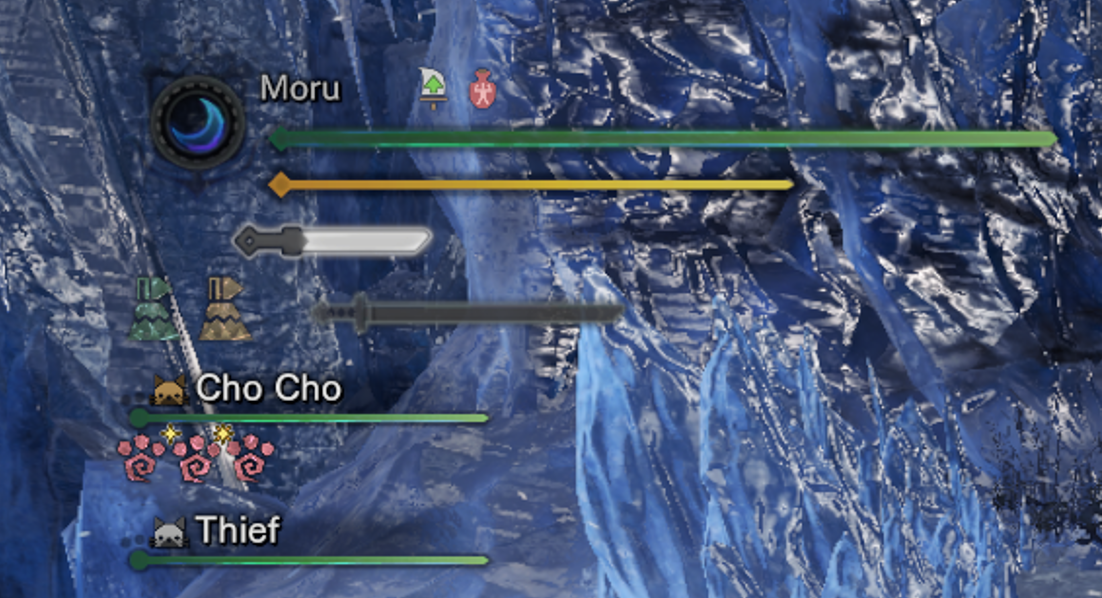
\includegraphics[width=\textwidth]{Image/HUD_Details/HP_Maximize.png}
        \captionof{figure}{Health Bar dan Stamina Bar dalam Battle Mode}
    \end{minipage}
    \end{center}
    \vspace{0.3cm}

    \item[Weapon Sharpness] Indikator warna pada ikon senjata membantu pemain mempersepsikan tingkat efektivitas serangan secara cepat.

    \item[Button/Combo Hint] Tampilan tombol di sisi kanan bawah layar memberikan petunjuk kombinasi serangan yang dapat digunakan, membantu pemain mempelajari kontrol tanpa perlu menghafal semua kombinasi.
      
    \begin{center}
        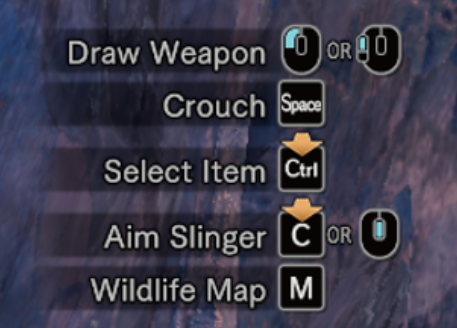
\includegraphics[width=0.8\textwidth]{Image/HUD_Details/Button_Hint.png}
        \captionof{figure}{Tampilan Button/Comobo Hint.}
    \end{center}

    \item[Item Wheel] Item Wheel menampilkan daftar cepat item seperti Potion, Trap, atau Bomb. Desain horizontal di bagian bawah layar memudahkan pemain memilih item dengan cepat tanpa membuka menu penuh. Pemain mempersepsikan bentuk ikon dan warna latar untuk mengenali fungsi item secara instan.
    
    \begin{center}
        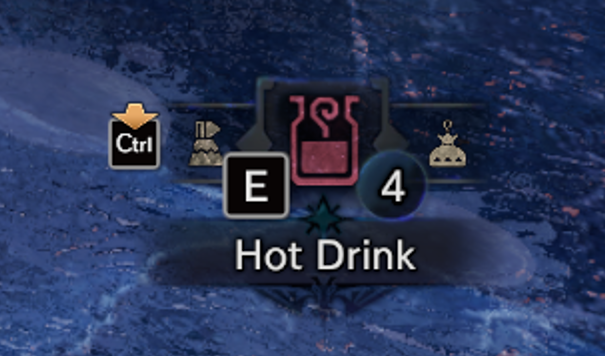
\includegraphics[width=0.8\textwidth]{Image/HUD_Details/Item_Wheel.png}
        \captionof{figure}{Tampilan Item Wheel.}
    \end{center}

    \item[Minimap] Minimap membantu pemain mempersepsikan posisi diri, arah monster, dan area penting di peta. Warna merah menandakan bahaya (monster agresif), sedangkan titik biru menandakan posisi rekan tim.  
    Desain visual minimap ini mendukung spatial perception (persepsi spasial) agar pemain selalu memahami situasi lingkungan sekitar.

    \begin{center}
        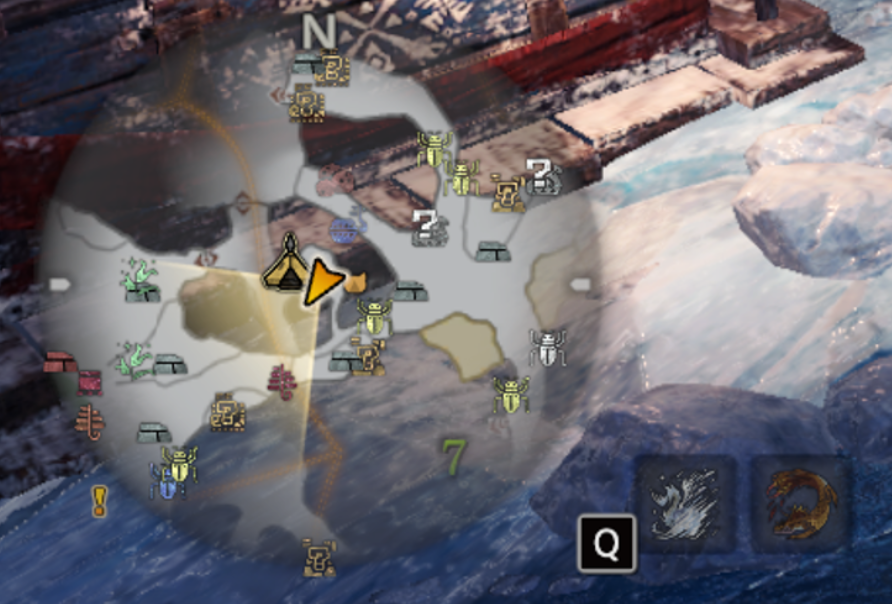
\includegraphics[width=0.8\textwidth]{Image/HUD_Details/Minimap.png}
        \captionof{figure}{Minimap.}
    \end{center}
\end{description}



\subsection{Atensi}
Monster Hunter: World secara aktif menarik atensi baik di menu maupun dalam game ke element penting dalam game.
Seperti Beberapa mekanik yang menarik atensi player seperti:
\begin{description}
    \item[Scoutfly] Efek visual berbentuk cahaya yang memandu pemain ke objective tertentu seperti loot, Area, Maupun Monster.
    \begin{center}
        \begin{minipage}{0.45\textwidth}
            \centering
            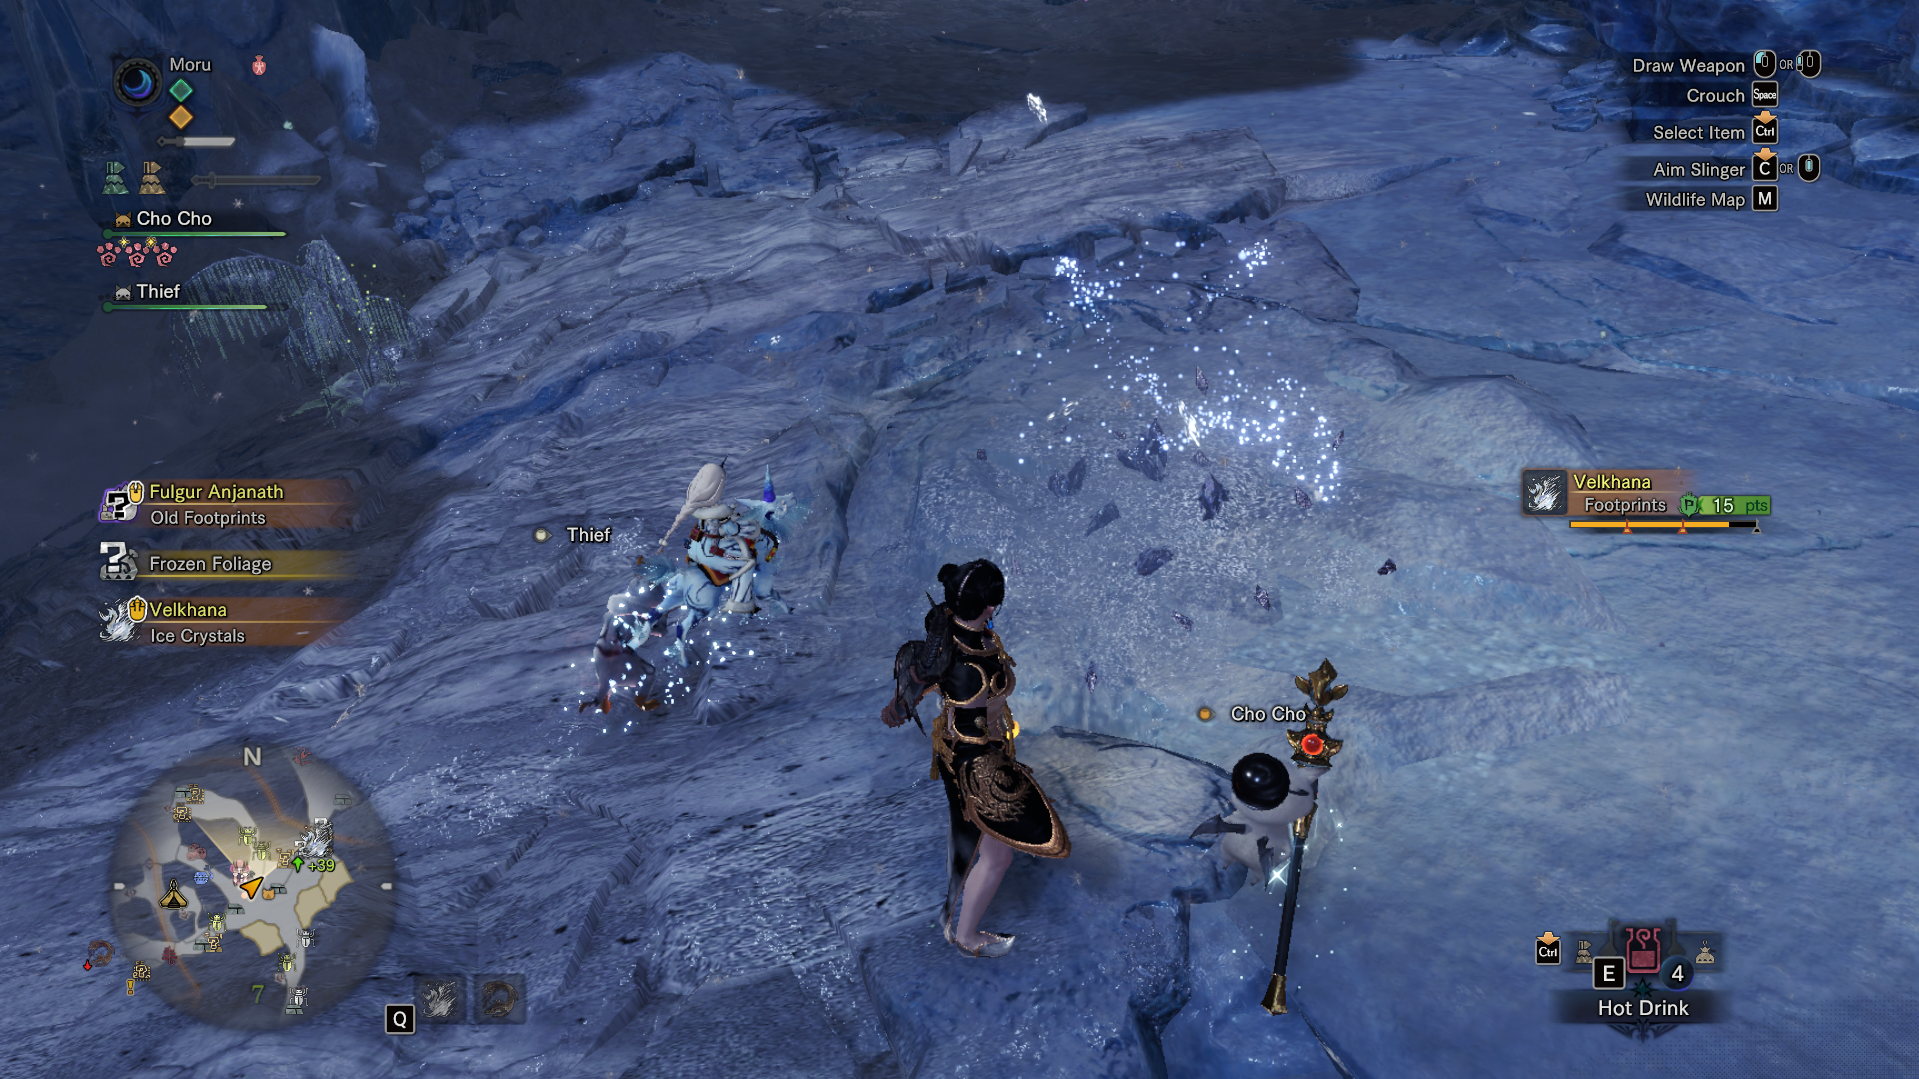
\includegraphics[width=\textwidth]{Image/Blue_Scoutfly.png}
            \captionof{figure}{Scoutfly Biru}
        \end{minipage}
        \hfill
        \begin{minipage}{0.45\textwidth}
            \centering
            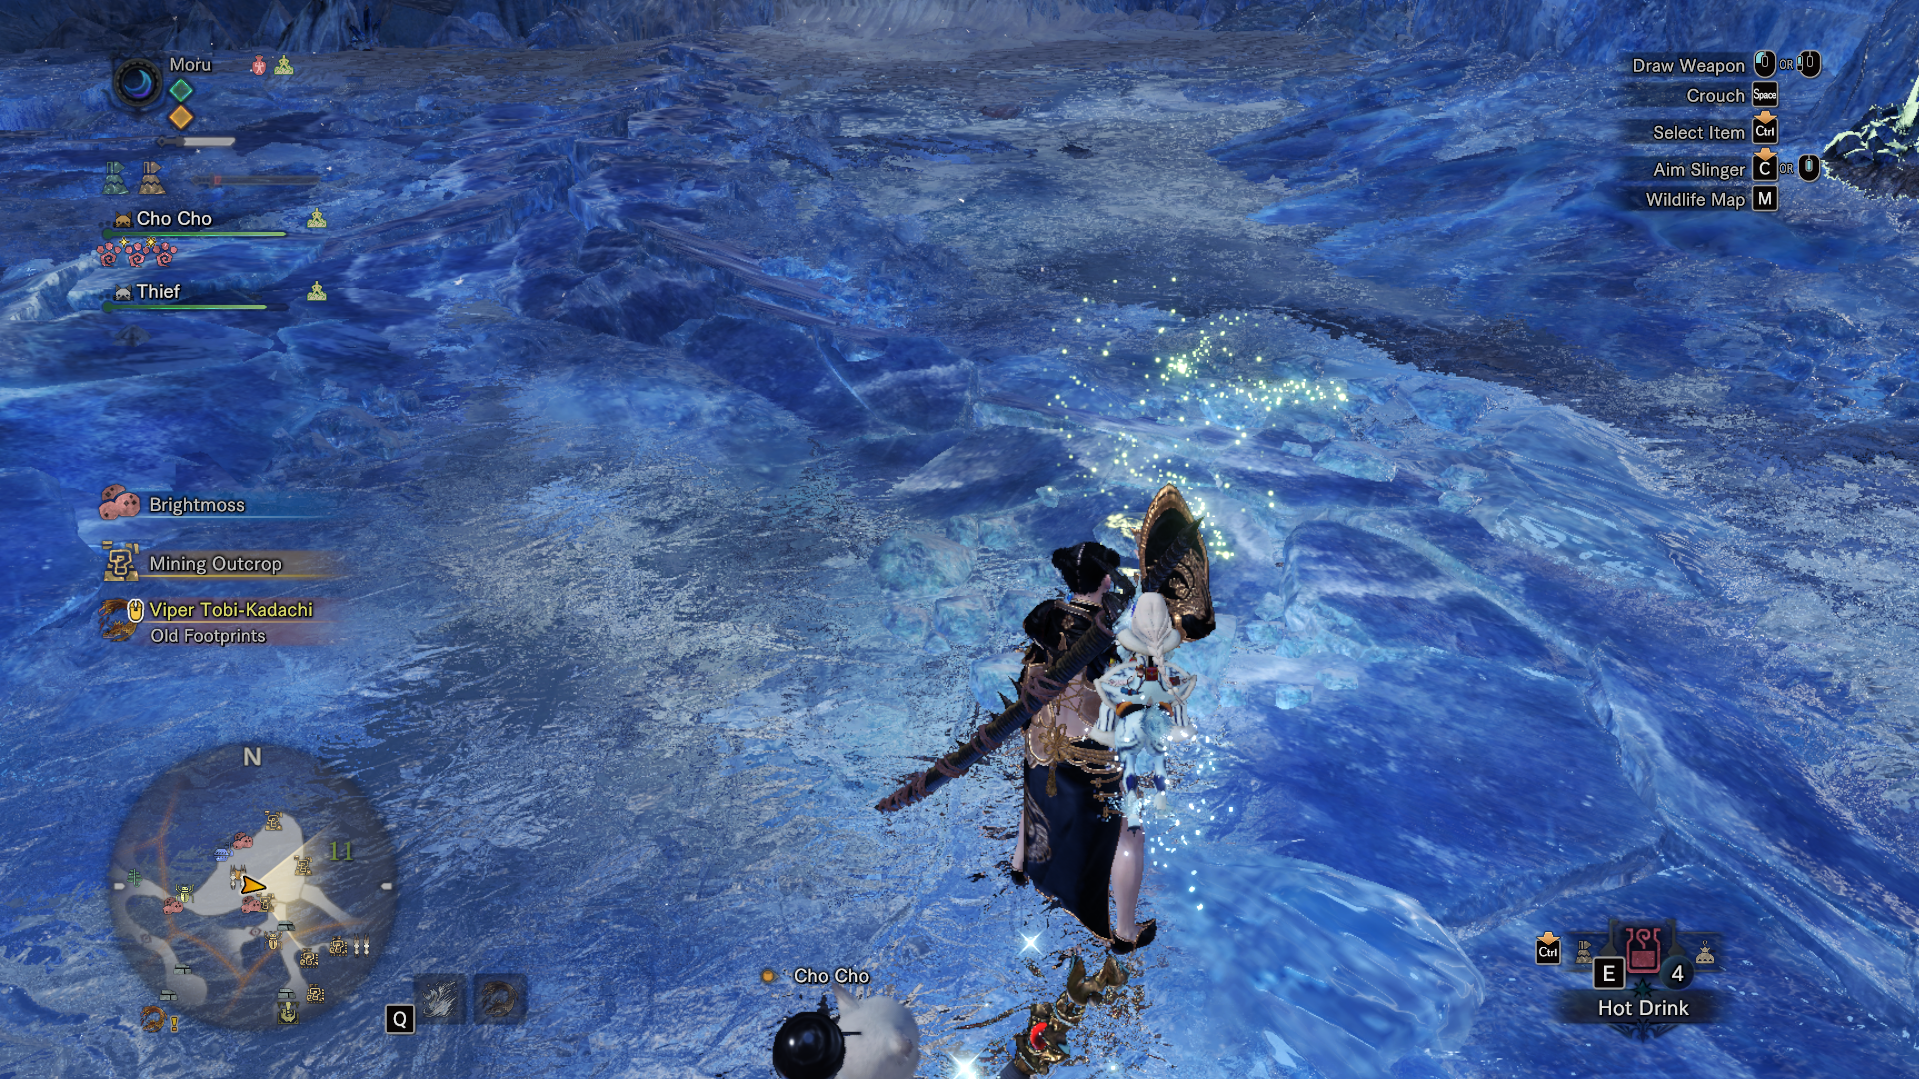
\includegraphics[width=\textwidth]{Image/Green_Scoutfly.png}
            \captionof{figure}{Scoutfly Hijau}
        \end{minipage}
    \end{center}
    \begin{center}
        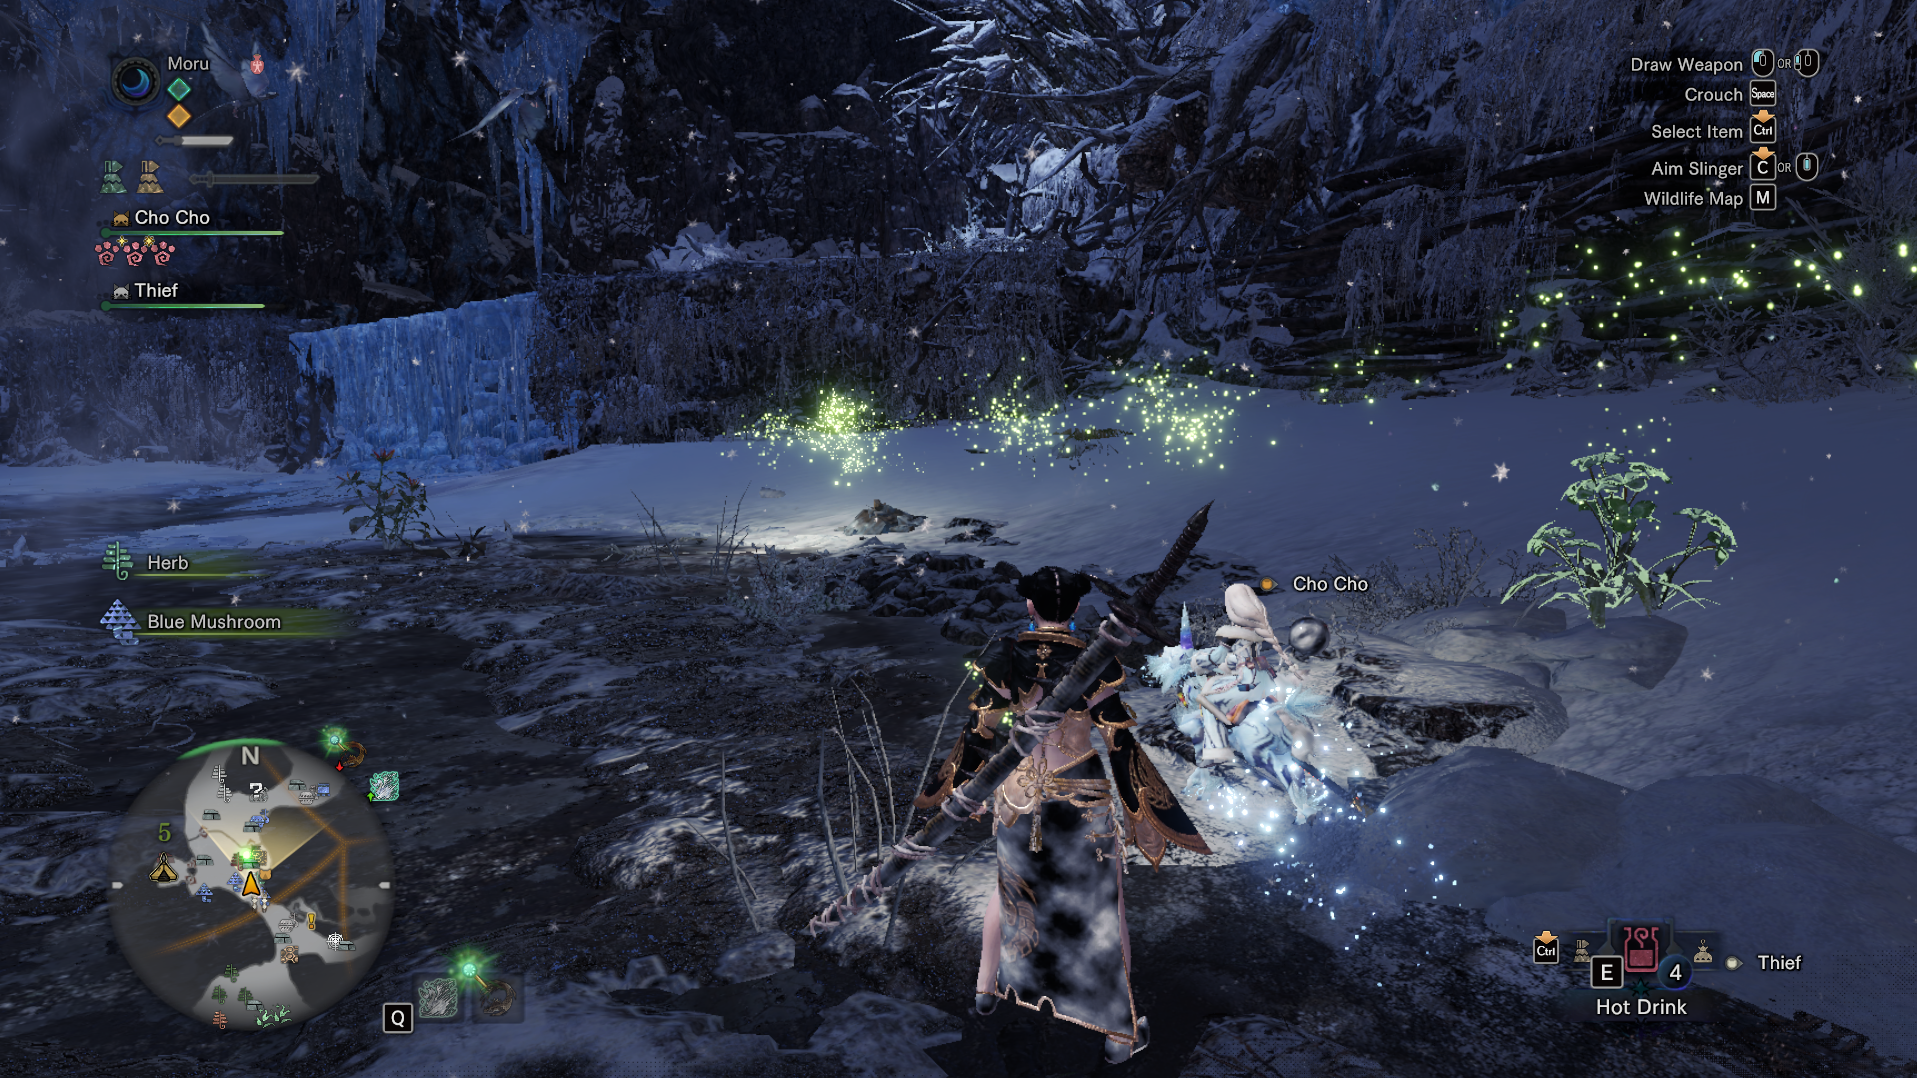
\includegraphics[width=0.8\textwidth]{Image/Scoutfly_Trail.png}
        \captionof{figure}{Jejak Scoutfly Mengarah Ke Objektif}
    \end{center}

    \item[Sound Cue] Selain elemen visual, Monster Hunter World menggunakan sound cue untuk mendukung atensi auditori.
    Raungan monster, perubahan musik latar, dan bunyi peringatan saat health rendah berfungsi mengarahkan fokus pemain secara otomatis tanpa perlu melihat tampilan HUD.\@
    Sistem ini efektif untuk memperkuat situational awareness dan mengurangi ketergantungan pada informasi visual. 
\end{description}

\subsection{Memori}
Pada Monster Hunter: World, Icon item dan monster juga berperan penting dalam proses memori visual pemain.Contohnya seperti botol hijau untuk Potion, dan jaring untuk Trap membantu pemain Mengenali Funsi Item secara cepat tanpa membaca teks.
Desain ikon yang konsisten juga membantu mendukung prinsip recognition over recall, sehingga pemain cukup mengenali simbol tanpa harus mengingat nama item atau monster. Dalam Monster Hunter Juga terdapat Hunters Note yang membantu pemain untuk Lebih mengenail Monster yang akan di lawan
\begin{center}
    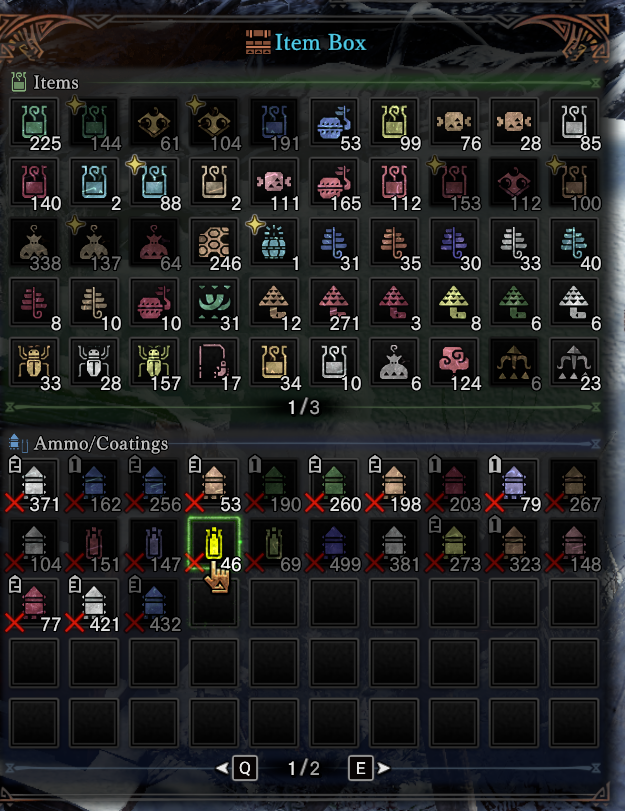
\includegraphics[width=0.8\textwidth]{Image/Item_List.png}
    \captionof{figure}{Item List dalam Box}
\end{center}
\begin{center}
    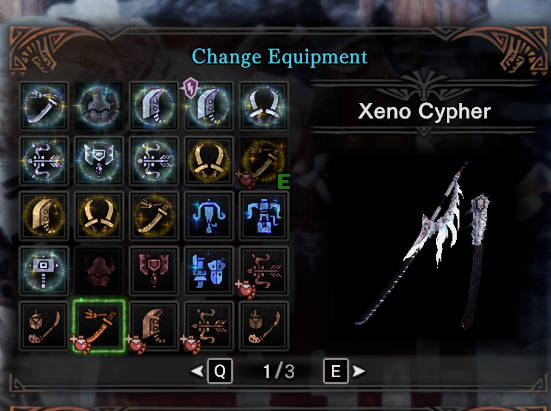
\includegraphics[width=0.8\textwidth]{Image/Gear_List.png}
    \captionof{figure}{Gear List dalam Box}
\end{center}
\begin{center}
    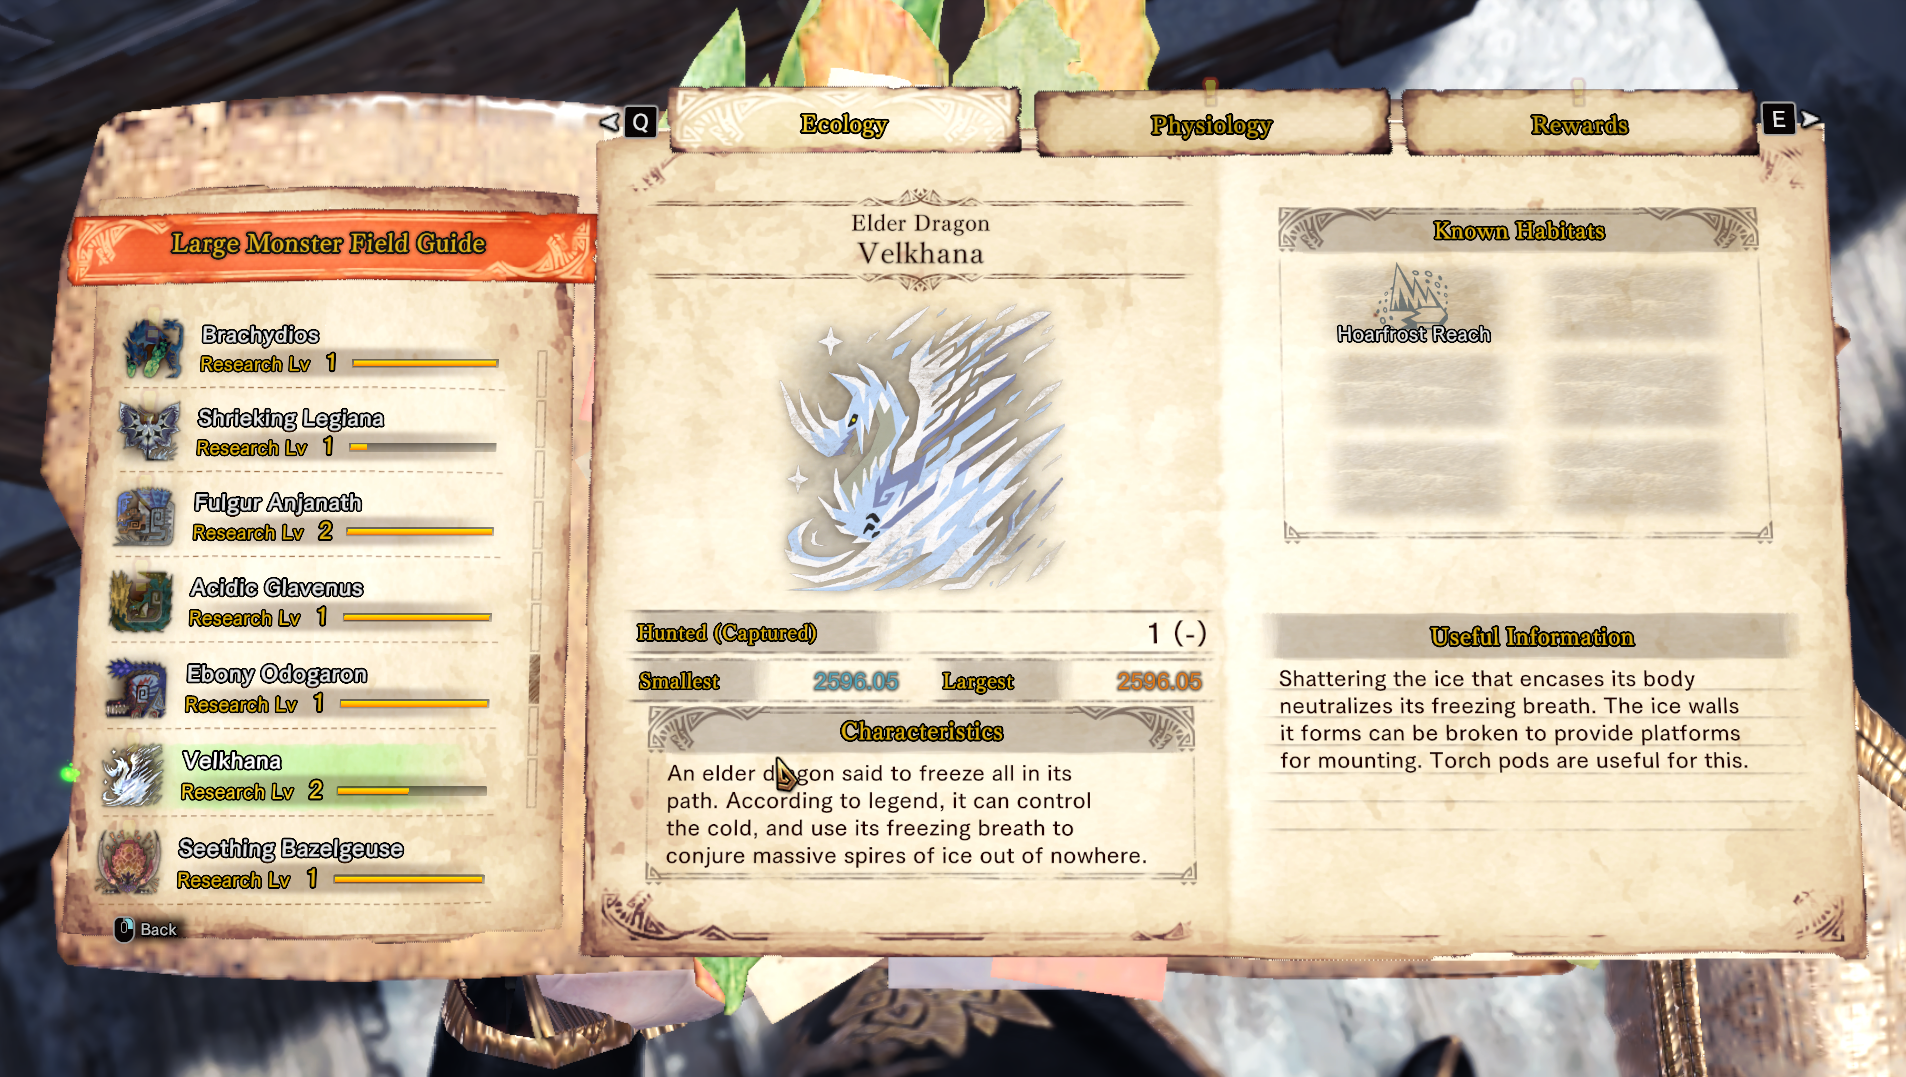
\includegraphics[width=0.8\textwidth]{Image/Hunters_Note.png}
    \captionof{figure}{Hunter's Note}
\end{center}


\subsection{Pengambilan Keputusan}
Dalam Monster Hunter: World, pemain terus-menerus dihadapkan pada proses pengambilan keputusan cepat berdasarkan kondisi pertempuran yang dinamis. Proses ini melibatkan integrasi antara persepsi visual, memori pengalaman, dan penilaian risiko. Contohnya, ketika health bar pemain tinggal sedikit, ia harus memutuskan apakah akan segera meminum Potion untuk memulihkan diri atau menunggu waktu yang lebih aman. Keputusan ini dipengaruhi oleh persepsi situasi (apakah monster sedang menyerang atau tidak), pengalaman sebelumnya, serta peluang untuk bertahan hidup.

Selain itu, pemain juga harus menentukan strategi pertempuran, seperti memilih kapan menyerang, menghindar, atau menggunakan jebakan. Pemain berpengalaman biasanya mengambil keputusan lebih cepat karena telah menyimpan pola perilaku monster dalam memori jangka panjang, sementara pemain baru cenderung mengalami decision delay akibat beban informasi yang tinggi. Desain visual dan audio yang responsif seperti perubahan musik saat monster marah atau ikon tengkorak yang menandakan monster hampir mati membantu pemain membuat keputusan berdasarkan recognition daripada analisis mendalam.

Dengan demikian, sistem umpan balik yang jelas dan konsisten dalam MHW mendukung proses pengambilan keputusan berbasis pengalaman, mengurangi beban kognitif, dan memungkinkan pemain merespons situasi dengan cepat dan tepat.

\section{Analisis Tugas (Task Analysis)}

\subsection{Tugas Utama: Crafting Senjata}

Tugas utama yang dianalisis dalam Monster Hunter World (MHW) adalah melakukan crafting (pembuatan) senjata baru di bengkel (Smithy). Proses ini melibatkan beberapa langkah yang dilakukan pemain mulai dari membuka area hub hingga senjata berhasil dibuat. Analisis ini menggambarkan urutan langkah, struktur hierarkis tugas, serta potensi masalah kognitif yang dapat muncul di tiap tahap.

Pertama, pemain masuk ke area Astera atau Seliana dan harus menuju ke lokasi Smithy tempat pembuatan senjata dilakukan. Bagi pemain baru, langkah ini dapat menimbulkan masalah memori spasial, karena pemain perlu mengingat lokasi NPC Smithy di antara banyak area yang berbeda. Setelah menemukan Smithy, pemain berinteraksi dengan NPC dan membuka menu “Craft Equipment”, yang merupakan langkah utama untuk memulai proses crafting.

Langkah berikutnya adalah memilih tipe senjata yang ingin dibuat (misalnya Great Sword atau Bow). Menu ini relatif mudah karena kategori ditampilkan dengan ikon dan teks yang jelas. Namun, ketika pemain menelusuri pohon senjata (Weapon Tree) untuk mencari varian tertentu, muncul potensi beban kognitif tinggi akibat banyaknya cabang dan informasi statistik yang harus dibandingkan. Pemain perlu menyeimbangkan keputusan antara kekuatan, elemen, dan ketersediaan material.

Setelah memilih senjata, pemain memeriksa daftar material yang dibutuhkan. Jika bahan tidak lengkap, pemain perlu mengingat jenis material dan sumbernya (misalnya: “Anjanath Fang ×2, Monster Bone+ ×3”), lalu beralih ke misi perburuan untuk mendapatkannya. Hal ini dapat menimbulkan beban memori kerja karena informasi tersebut harus diingat saat keluar dari menu. Setelah bahan lengkap, pemain kembali ke Smithy untuk melakukan crafting dan mengonfirmasi pembuatan senjata, menandakan tugas selesai.

Secara keseluruhan, proses ini menggambarkan hubungan antara persepsi, memori, dan pengambilan keputusan dalam konteks tugas kompleks. Desain visual yang jelas dan struktur menu yang konsisten membantu pemain mengurangi beban kognitif, namun kompleksitas pohon senjata dan banyaknya informasi tetap menjadi tantangan utama bagi pengguna baru.



\subsection{Potensi Masalah Kognitif}

\begin{itemize}
\item Pergi ke Smithy: Pemain baru dapat mengalami beban memori spasial karena harus mengingat lokasi NPC di area yang luas dan bertingkat.
\item Menelusuri Pohon Senjata: Dapat menimbulkan beban kognitif tinggi karena banyaknya pilihan dan informasi statistik yang kompleks.
\item Memeriksa Material: Potensi masalah persepsi akibat ikon material yang kecil serta beban memori kerja ketika harus mengingat bahan yang kurang.
\item Proses Crafting: Risiko kesalahan klik (misclick) jika pemain terlalu cepat menekan tombol konfirmasi tanpa memeriksa ulang.
\end{itemize}

\subsection{Diagram HTA}

\begin{center}
    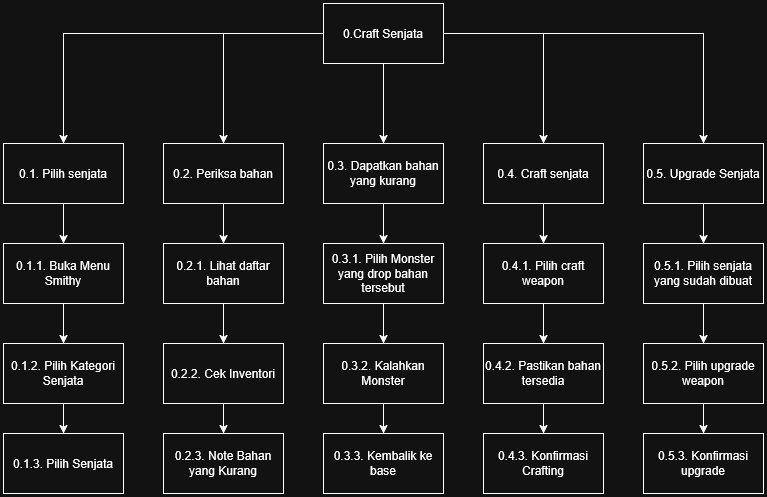
\includegraphics[width=0.8\textwidth]{Image/HTA.png}
    \captionof{figure}{Diagram HTA}
\end{center}


\end{document}
